\section{Technical Appendices and Supplementary Material}
In this section, we present the automated evaluation results, employing GPT-4.1 as the evaluation expert. This analysis aims to provide researchers with deeper insights into the characteristics of our dataset, as well as the variations in outcomes attributable to different evaluation experts. Additionally, we include the original caption outputs and corresponding evaluation results produced by various models for comprehensive comparison.


\subsection{More Experimental Results With GPT-4.1}\label{exp_app}

\begin{table*}[htbp]
\renewcommand{\arraystretch}{0.6}
\caption{The accuracy (AR), inconsistency rate (IR), and coverage rate (CR) of VLM methods on all dimensions, where GPT-4.1 as a TextQA expert. The symbol ``$\uparrow$"  indicates that the larger the value, the better; The symbol ``$\downarrow$" indicates that the smaller the value, the better.}
\label{tab:results_2}
\resizebox{\textwidth}{!}{%
\begin{tabular}{@{}ll|cccccccccccc@{}}
\toprule
 &\multirow{3}{*}{Methods}& \multicolumn{7}{c|}{Content \& Entity}& \multicolumn{4}{c}{Color \&  Light}\\
 \cline{3-13} 
 &  & \begin{tabular}[c]{@{}c@{}}\small Proper\\ \small Noun\end{tabular} & \begin{tabular}[c]{@{}c@{}}Action\end{tabular} & \begin{tabular}[c]{@{}c@{}}Relation
\end{tabular} & \begin{tabular}[c]{@{}c@{}}Count
\end{tabular} & Entity  & \begin{tabular}[c]{@{}c@{}}\small Entity\\ \small Size\end{tabular} & \multicolumn{1}{c|}{\begin{tabular}[c]{@{}c@{}}\small Entity\\ \small Shape\end{tabular} }
&\begin{tabular}[c]{@{}c@{}}Lighting
\end{tabular} & \begin{tabular}[c]{@{}c@{}}\small Color \\ \small Palette \end{tabular} & \begin{tabular}[c]{@{}c@{}}\small Color\\ \small Grading
\end{tabular} & \begin{tabular}[c]{@{}c@{}}Color
\end{tabular}  \\ \midrule
\multirow{8}{*}{\rotatebox{90}{AR}$\Bigg\uparrow$} 
& LLaVA-Video-7B & 40.73 & 57.08 & 51.67 & 54.88 & 34.02 & 66.2 & \multicolumn{1}{c|}{26.62} & 57.59 & 61.49 & 23.78 & 55.97 \\
& Qwen2VL-7B & 39.17 & 56.32 & 52.87 & 57.17 & 32.27 & 64.2 & \multicolumn{1}{c|}{25.61} & 69.93 & 55.57 & 30.62 & \multicolumn{1}{c|}{50.75}  \\ 
& VideoLLaMA3-7B & 38.92 & 58.51 & 52.56 & 56.27 & 33.48 & 64.28 & \multicolumn{1}{c|}{25.56} & 60.59 & 59.03 & 25.24 & \multicolumn{1}{c|}{54.12}\\
& NVILA-8B & 40.03 & 44.2 & 48.04 & 57.9 & 37.3 & 63.72 & \multicolumn{1}{c|}{29.32} & 72.63 & 66.01 & 42.37 & \multicolumn{1}{c|}{59.35} \\ 
& InternVL2.5-8B & 38.63 & 53.86 & 48.71 & 59.64 & 36.78 & 60.91 & \multicolumn{1}{c|}{29.44} & 81.27 & 75.35 & 60.36 & \multicolumn{1}{c|}{55.82} \\
& Qwen2.5VL-7B & 46.95 & 63.86 & 57.72 & 62.39 & 41.75 & 69.35 & \multicolumn{1}{c|}{34.89} & 83.6 & 73.9 & 51.32 & \multicolumn{1}{c|}{59.8}  \\ 
& Qwen2.5-VL-72B & 48.76 & 67.28 & 63.03 & 67.33 & 45.37 & 72.51 & \multicolumn{1}{c|}{37.76} & 88.42 & 75.28 & 61.31 & \multicolumn{1}{c|}{62.69}  \\ 
& GPT-4o  & 51.11 & 69.48 & 66.34 & 70.08 & 51.38 & 77.5 & \multicolumn{1}{c|}{47.89} & 87.96 & 82.47 & 68.17 & \multicolumn{1}{c|}{67.07} \\ 
& Gemini2.5-Pro-Flash & 60.21 & 76.23 & 73.54 & 79.59 & 63.97 & 85.25 & \multicolumn{1}{c|}{59.55} & \textbf{90.05} & 86.57 & \textbf{69.06} & \multicolumn{1}{c|}{79.36}\\ 
& Gemini-2.5-Pro-Preview & \textbf{61.41} & \textbf{78.13} & \textbf{75.19} & \textbf{80.54} & \textbf{64.4} & \textbf{86.52} & \multicolumn{1}{c|}{\textbf{62.21}} & 88.9 & \textbf{88.06} & 66.95 & \multicolumn{1}{c|}{\textbf{79.96}} \\ 

\midrule
\multirow{8}{*}{\rotatebox{90}{IR}$\Bigg\downarrow$} 
& LLaVA-Video-7B & 13.09 & 15.13 & 11.29 & 13.14 & 3.76 & 8.62 & \multicolumn{1}{c|}{8.45} & \textbf{5.62} & 11.05 & \textbf{4.12} & \multicolumn{1}{c|}{13.23} \\
& Qwen2VL-7B & 8.38 & 13.84 & 10.27 & 11.67 & 3.77 & 8.64 & \multicolumn{1}{c|}{\textbf{6.05}} & 7.26 & 12.88 & 5.67 & \multicolumn{1}{c|}{13.44} \\
& VideoLLaMA3-7B & 9.91 & 17.88 & 11.99 & 12.59 & 3.46 & 8.41 & \multicolumn{1}{c|}{7.56} & 6.19 & 11.49 & 4.39 & \multicolumn{1}{c|}{12.77}  \\
& NVILA-8B & 11.88 & 20.21 & 14.96 & 15.45 & 4.48 & 12.42 & \multicolumn{1}{c|}{9.61} & 8.08 & 15.72 & 6.52 & \multicolumn{1}{c|}{17.75}  \\
& InternVL2.5-8B & 14.57 & 19.0 & 16.43 & 14.18 & 5.5 & 14.0 & \multicolumn{1}{c|}{10.23} & 8.06 & 15.11 & 8.57 & \multicolumn{1}{c|}{16.01} \\
& Qwen2.5VL-7B & 8.65 & 14.66 & 12.39 & 11.35 & \textbf{3.16} & 9.25 & \multicolumn{1}{c|}{8.38} & 6.9 & 11.5 & 5.52 & \multicolumn{1}{c|}{13.87} \\

& Qwen2.5-VL-72B & 7.86 & 15.0 & 11.58 & 11.66 & 5.02 & 8.96 & \multicolumn{1}{c|}{8.28} & 6.89 & 13.44 & 5.3 & \multicolumn{1}{c|}{15.23} \\ 
& GPT-4o & 7.53 & \textbf{11.26} & \textbf{9.56} & 10.45 & 3.94 & 6.5 & \multicolumn{1}{c|}{8.48} & 6.34 & 11.69 & 7.32 & \multicolumn{1}{c|}{13.15} \\ 
& Gemini2.5-Pro-Flash & 6.76 & 12.59 & 9.57 & 9.81 & 5.23 & \textbf{5.36} & \multicolumn{1}{c|}{8.43} & 6.43 & 11.32 & 6.98 & \multicolumn{1}{c|}{\textbf{11.19}} \\
& Gemini-2.5-Pro-Preview & \textbf{6.58}& 13.06 & 9.77 & \textbf{9.06} & 4.29 & 5.88 & \multicolumn{1}{c|}{8.64} & 7.08 & \textbf{10.16} & 5.76 & \multicolumn{1}{c|}{12.18}\\ 

 \midrule
\multirow{8}{*}{\rotatebox{90}{CR}$\Bigg\uparrow$} 
& LLaVA-Video-7B & 46.87 & 67.25 & 58.25 & 63.17 & 35.35 & 72.44 & \multicolumn{1}{c|}{29.07} & 61.03 & 69.13 & 24.81 & \multicolumn{1}{c|}{64.51}   \\
& Qwen2VL-7B & 42.75 & 65.36 & 58.92 & 64.73 & 33.54 & 70.27 & \multicolumn{1}{c|}{27.26} & 75.41 & 63.79 & 32.46 & \multicolumn{1}{c|}{58.63}  \\ 
& VideoLLaMA3-7B & 43.2 & 71.25 & 59.72 & 64.38 & 34.68 & 70.19 & \multicolumn{1}{c|}{27.65} & 64.59 & 66.7 & 26.4 & \multicolumn{1}{c|}{62.05}  \\
& NVILA-8B & 45.43 & 55.4 & 56.49 & 68.48 & 39.05 & 72.76 & \multicolumn{1}{c|}{32.43} & 79.01 & 78.33 & 45.32 & \multicolumn{1}{c|}{72.16}  \\
& InternVL2.5-8B & 45.22 & 66.49 & 58.29 & 69.49 & 38.92 & 70.82 & \multicolumn{1}{c|}{32.8} & 88.4 & 88.75 & 66.02 & \multicolumn{1}{c|}{66.46}   \\
& Qwen2.5VL-7B & 51.4 & 74.83 & 65.88 & 70.37 & 43.11 & 76.42 & \multicolumn{1}{c|}{38.08} & 89.79 & 83.5 & 54.32 & \multicolumn{1}{c|}{69.43} \\ 
& Qwen2.5-VL-72B & 52.92 & 79.16 & 71.28 & 76.21 & 47.76 & 79.64 & \multicolumn{1}{c|}{41.17} & 94.96 & 86.97 & 64.74 & \multicolumn{1}{c|}{73.96}  \\ 

& GPT-4o & 55.27 & 78.3 & 73.36 & 78.26 & 53.48 & 82.89 & \multicolumn{1}{c|}{52.33} & 93.92 & 93.39 & 73.56 & \multicolumn{1}{c|}{77.23}\\ 
& Gemini2.5-Pro-Flash & 64.58 & 87.22 & 81.32 & 88.25 & \textbf{67.5} & 90.07 & \multicolumn{1}{c|}{65.03} & \textbf{96.24} & 97.62 & \textbf{74.24} & \multicolumn{1}{c|}{89.36}\\ 
& Gemini-2.5-Pro-Preview & \textbf{65.73} & \textbf{89.86} & \textbf{83.33} & \textbf{88.56} & 67.28 & \textbf{91.93} & \multicolumn{1}{c|}{\textbf{68.1}} & 95.68 & \textbf{98.02} & 71.04 & \multicolumn{1}{c|}{\textbf{91.04}} \\ 


 \bottomrule
 \toprule
 &\multirow{3}{*}{Methods}& \multicolumn{5}{c|}{Visuals \& Composition}& \multicolumn{5}{c|}{Cinematography  \& Environment}\\
 \cline{3-13} 
 &  & Position & \begin{tabular}[c]{@{}c@{}}\small Relative\\ \small Position\end{tabular} & Background &Text & \multicolumn{1}{c|}{Blur} & Style & \begin{tabular}[c]{@{}c@{}}\small Camera \\ \small Movement\end{tabular} & \begin{tabular}[c]{@{}c@{}}Shot Type\end{tabular} & \begin{tabular}[c]{@{}c@{}}Emotion\end{tabular} & \multicolumn{1}{c|}{Atmosphere} & \color{red}\textbf{ALL}\\ \midrule
\multirow{8}{*}{\rotatebox{90}{AR}$\Bigg\uparrow$} 

& LLaVA-Video-7B & 34.26 & 32.96 & 69.28 & 43.75 & \multicolumn{1}{c|}{13.49} & 66.6 & 23.68 & 38.13 & 48.53 & \multicolumn{1}{c|}{82.04} & 47.74 \\
& Qwen2VL-7B & 35.34 & 32.4 & 68.69 & 34.75 & \multicolumn{1}{c|}{15.17} & 71.53 & 16.26 & 32.7 & 55.24 & \multicolumn{1}{c|}{83.56} & 47.45\\ 
& VideoLLaMA3-7B & 35.41 & 32.54 & 65.35 & 38.11 & \multicolumn{1}{c|}{16.99} & 71.66 & 39.32 & 39.53 & 53.27 & \multicolumn{1}{c|}{80.44} &48.45  \\
& NVILA-8B & 40.69 & 33.36 & 69.7 & 38.04 & \multicolumn{1}{c|}{26.42} & 74.11 & 16.97 & 39.4 & 53.46 & \multicolumn{1}{c|}{81.02} &49.70 \\
& InternVL2.5-8B & 39.08 & 32.59 & 70.89 & 37.31 & \multicolumn{1}{c|}{36.83} & 86.59 & 51.3 & 50.53 & 58.75 & \multicolumn{1}{c|}{86.57} &54.85  \\
 & Qwen2.5VL-7B & 45.0 & 38.58 & 77.18 & 44.96 & \multicolumn{1}{c|}{30.71} & 88.55 & 51.92 & 50.9 & 63.5 & \multicolumn{1}{c|}{89.51} &58.74 \\ 
& Qwen2.5-VL-72B & 49.83 & 43.01 & 78.99 & 45.55 & \multicolumn{1}{c|}{36.31} & 92.0 & 66.47 & 59.37 & 67.78 & \multicolumn{1}{c|}{89.91} &63.08 \\
& GPT-4o & 57.24 & 49.0 & 83.14 & 46.79 & \multicolumn{1}{c|}{48.0} & 92.05 & 55.57 & 62.97 & 62.45 & \multicolumn{1}{c|}{\textbf{90.82}} &66.49\\
& Gemini2.5-Pro-Flash & 70.36 & 63.56 & 87.64 & \textbf{63.7} & \multicolumn{1}{c|}{67.33} & \textbf{96.13} & 70.76 & 74.29 & 73.01 & \multicolumn{1}{c|}{86.22} &75.56 \\
& Gemini-2.5-Pro-Preview & \textbf{70.63} & \textbf{66.11} & \textbf{87.97} & 63.5 & \multicolumn{1}{c|}{\textbf{68.75}} & 95.76 & \textbf{74.89} & \textbf{75.72} & \textbf{77.05} & \multicolumn{1}{c|}{88.34} &\color{red}\textbf{76.73}\\


 \midrule
\multirow{8}{*}{\rotatebox{90}{IR}$\Bigg\downarrow$} 
& LLaVA-Video-7B & \textbf{10.46} & 11.83 & 7.5 & 17.92 & \multicolumn{1}{c|}{\textbf{10.11}} & \textbf{1.64} & 24.13 & \textbf{12.18} & \textbf{3.67} & \multicolumn{1}{c|}{\textbf{3.71}} & 10.05\\
& Qwen2VL-7B & 11.18 & \textbf{10.39} & 8.8 & 13.47 & \multicolumn{1}{c|}{14.47} & 2.72 & 19.21 & 13.17 & 5.16 & \multicolumn{1}{c|}{6.25} & \color{red}\textbf{9.65} \\
& VideoLLaMA3-7B & 12.26 & 12.21 & 7.94 & 14.86 & \multicolumn{1}{c|}{12.18} & 2.22 & 23.44 & 14.68 & 3.74 & \multicolumn{1}{c|}{4.52} &10.50\\
& NVILA-8B & 16.22 & 16.46 & 10.26 & 17.93 & \multicolumn{1}{c|}{18.62} & 4.51 & 23.6 & 22.5 & 6.31 & \multicolumn{1}{c|}{6.05} &13.12\\
& InternVL2.5-8B & 15.32 & 14.72 & 8.74 & 19.13 & \multicolumn{1}{c|}{21.88} & 4.89 & 26.24 & 20.04 & 6.11 & \multicolumn{1}{c|}{5.57} &13.41 \\
& Qwen2.5VL-7B & 12.8 & 13.45 & 8.37 & 12.25 & \multicolumn{1}{c|}{19.8} & 2.72 & 22.77 & 16.43 & 5.47 & \multicolumn{1}{c|}{5.09} & 10.62\\

& Qwen2.5-VL-72B & 13.34 & 13.5 & 7.98 & 12.56 & \multicolumn{1}{c|}{20.73} & 3.36 & 20.99 & 16.97 & 5.56 & \multicolumn{1}{c|}{5.14} &10.98\\
& GPT-4o & 12.42 & 12.35 & 6.23 & 12.9 & \multicolumn{1}{c|}{22.32} & 3.64 & 21.35 & 19.02 & 6.91 & \multicolumn{1}{c|}{5.06} &10.24\\

&  Gemini2.5-Pro-Flash & 14.68 & 15.16 & \textbf{5.05} & 11.87 & \multicolumn{1}{c|}{23.45} & 2.25 & 20.57 & 20.34 & 5.12 & \multicolumn{1}{c|}{4.79} &10.49\\

&Gemini-2.5-Pro-Preview & 15.65 & 13.98 & 5.12 & \textbf{10.92} & \multicolumn{1}{c|}{22.58} & 2.33 & \textbf{18.68} & 19.17 & 4.7 & \multicolumn{1}{c|}{4.7} &10.28\\

 \midrule
\multirow{8}{*}{\rotatebox{90}{CR}$\Bigg\uparrow$} 
& LLaVA-Video-7B & 38.26 & 37.38 & 74.9 & 53.3 & \multicolumn{1}{c|}{15.01} & 67.71 & 31.22 & 43.42 & 50.38 & \multicolumn{1}{c|}{85.2} & 53.08\\
& Qwen2VL-7B & 39.79 & 36.16 & 75.32 & 40.16 & \multicolumn{1}{c|}{17.74} & 73.53 & 20.13 & 37.66 & 58.25 & \multicolumn{1}{c|}{89.14}  & 52.52\\ 
& VideoLLaMA3-7B & 40.36 & 37.07 & 70.98 & 44.76 & \multicolumn{1}{c|}{19.35} & 73.29 & 51.37 & 46.33 & 55.34 & \multicolumn{1}{c|}{84.25}  & 54.13\\
& NVILA-8B & 48.57 & 39.93 & 77.67 & 46.35 & \multicolumn{1}{c|}{32.46} & 77.61 & 22.22 & 50.83 & 57.06 & \multicolumn{1}{c|}{86.24}  & 57.21\\
& InternVL2.5-8B & 46.15 & 38.22 & 77.69 & 46.14 & \multicolumn{1}{c|}{47.14} & 91.05 & 69.55 & 63.19 & 62.57 & \multicolumn{1}{c|}{91.68} & 63.34\\
& Qwen2.5VL-7B & 51.6 & 44.58 & 84.23 & 51.24 & \multicolumn{1}{c|}{38.3} & 91.03 & 67.23 & 60.91 & 67.17 & \multicolumn{1}{c|}{94.31} &65.75 \\
& Qwen2.5-VL-72B & 57.5 & 49.72 & 85.84 & 52.1 & \multicolumn{1}{c|}{45.81} & 95.2 & 84.14 & 71.51 & 71.78 & \multicolumn{1}{c|}{94.78} &70.86\\
& GPT-4o & 65.36 & 55.91 & 88.67 & 53.72 & \multicolumn{1}{c|}{61.8} & 95.52 & 70.65 & 77.77 & 67.09 & \multicolumn{1}{c|}{\textbf{95.66}} &74.07\\
& Gemini2.5-Pro-Flash & 82.47 & 74.92 & 92.3 & \textbf{72.27} & \multicolumn{1}{c|}{87.96} & \textbf{98.35} & 89.09 & 93.26 & 76.95 & \multicolumn{1}{c|}{90.55} &84.42\\
& Gemini-2.5-Pro-Preview & \textbf{83.74} & \textbf{76.86} & \textbf{92.72} & 71.28 & \multicolumn{1}{c|}{\textbf{88.8}} & 98.04 & \textbf{92.09} & \textbf{93.68} & \textbf{80.85} & \multicolumn{1}{c|}{92.7}&\color{red}\textbf{85.52} \\

\bottomrule
\end{tabular}%
}
\end{table*}

\begin{figure*}[tp]
	\begin{minipage}[t]{1.0\linewidth}
        \centering
	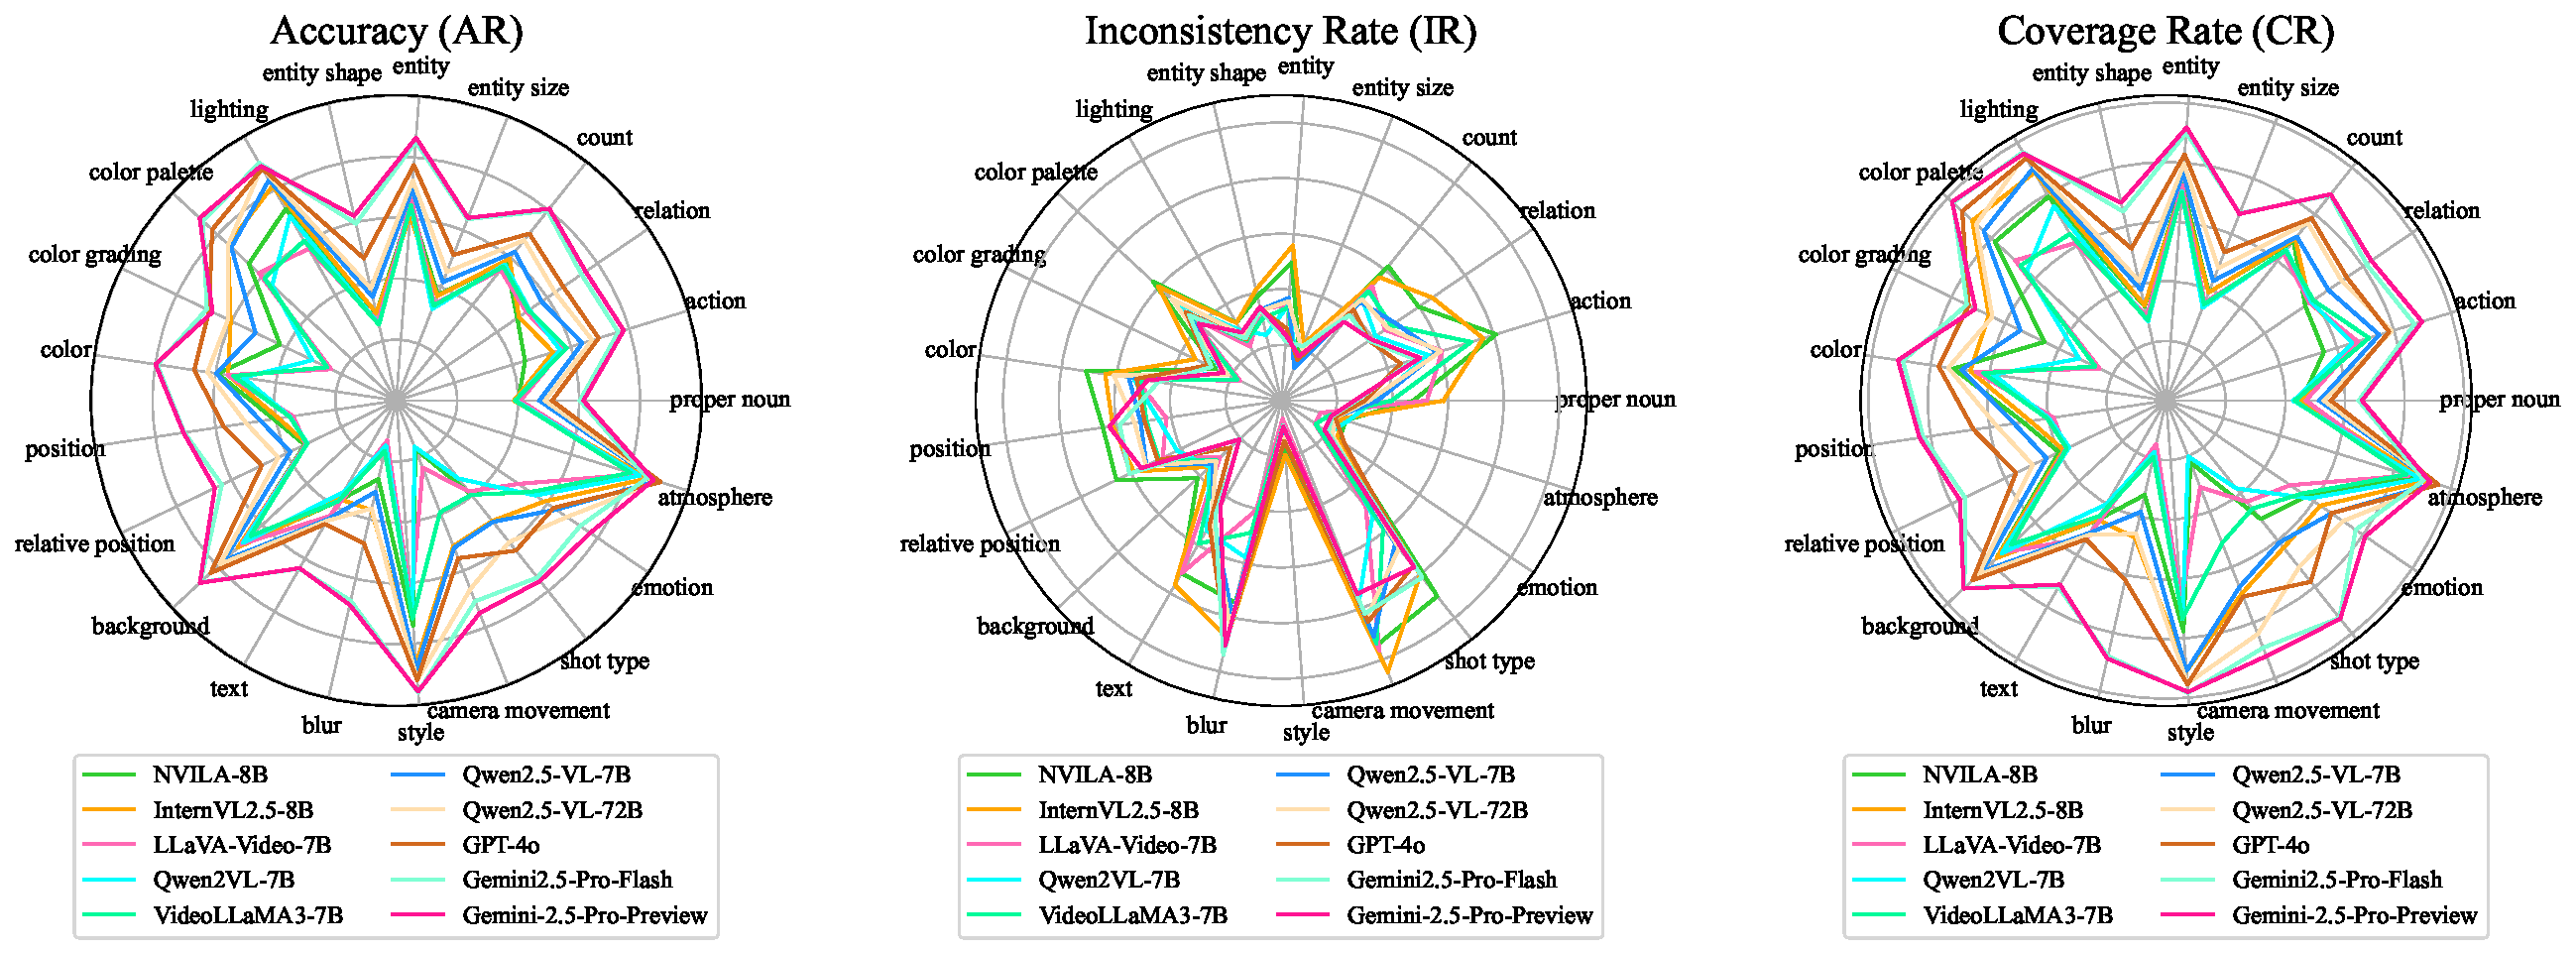
\includegraphics[width=1.0\linewidth]{imgs/radar_chart_all-New2.pdf}
	\caption{Results of GPT-4.1 captioning evaluation, organized by category.}
	\label{fig:fig9}
	\end{minipage}%
\end{figure*}

\begin{figure}[thbp]
	\begin{minipage}[t]{1.0\linewidth}
        \centering
	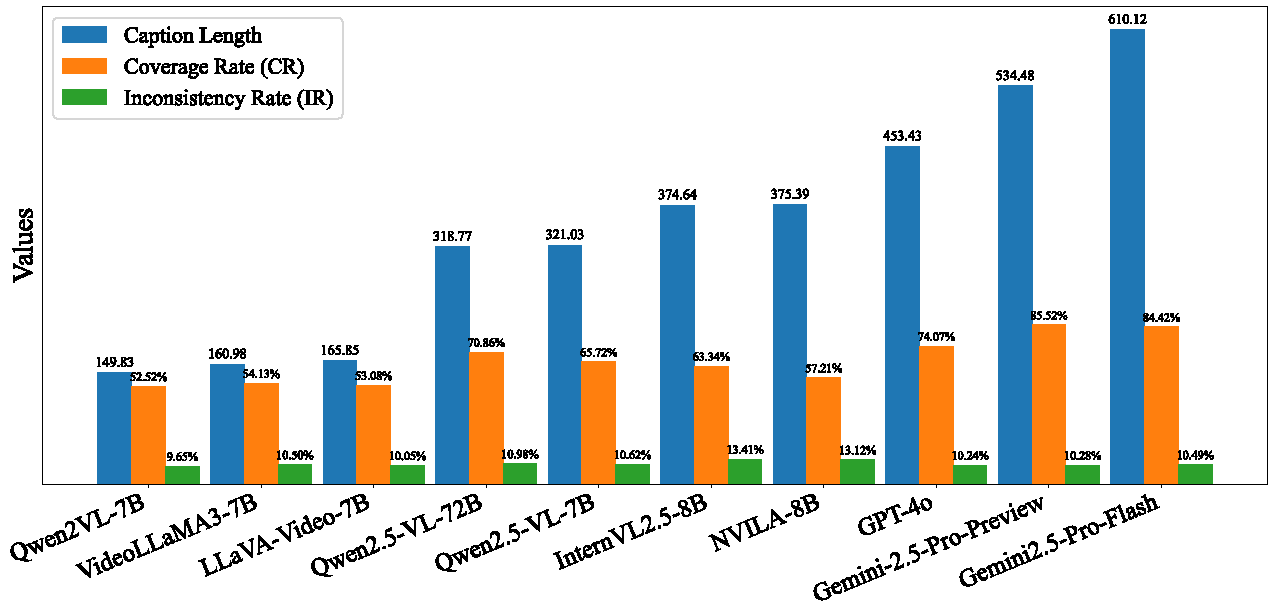
\includegraphics[width=0.9\linewidth]{imgs/comparison_chart_sorted_NEW22.pdf}
    \vspace{-0.5em}
	\caption{The relationship between CR, IR and caption length, where GPT-4.1 as a TextQA expert. Caption length is the number of words in the caption, not counting special symbols.}
	\label{fig:fig10}
	\end{minipage}%
\end{figure}

\begin{figure}[thbp]
	\begin{minipage}[t]{1.0\linewidth}
        \centering
	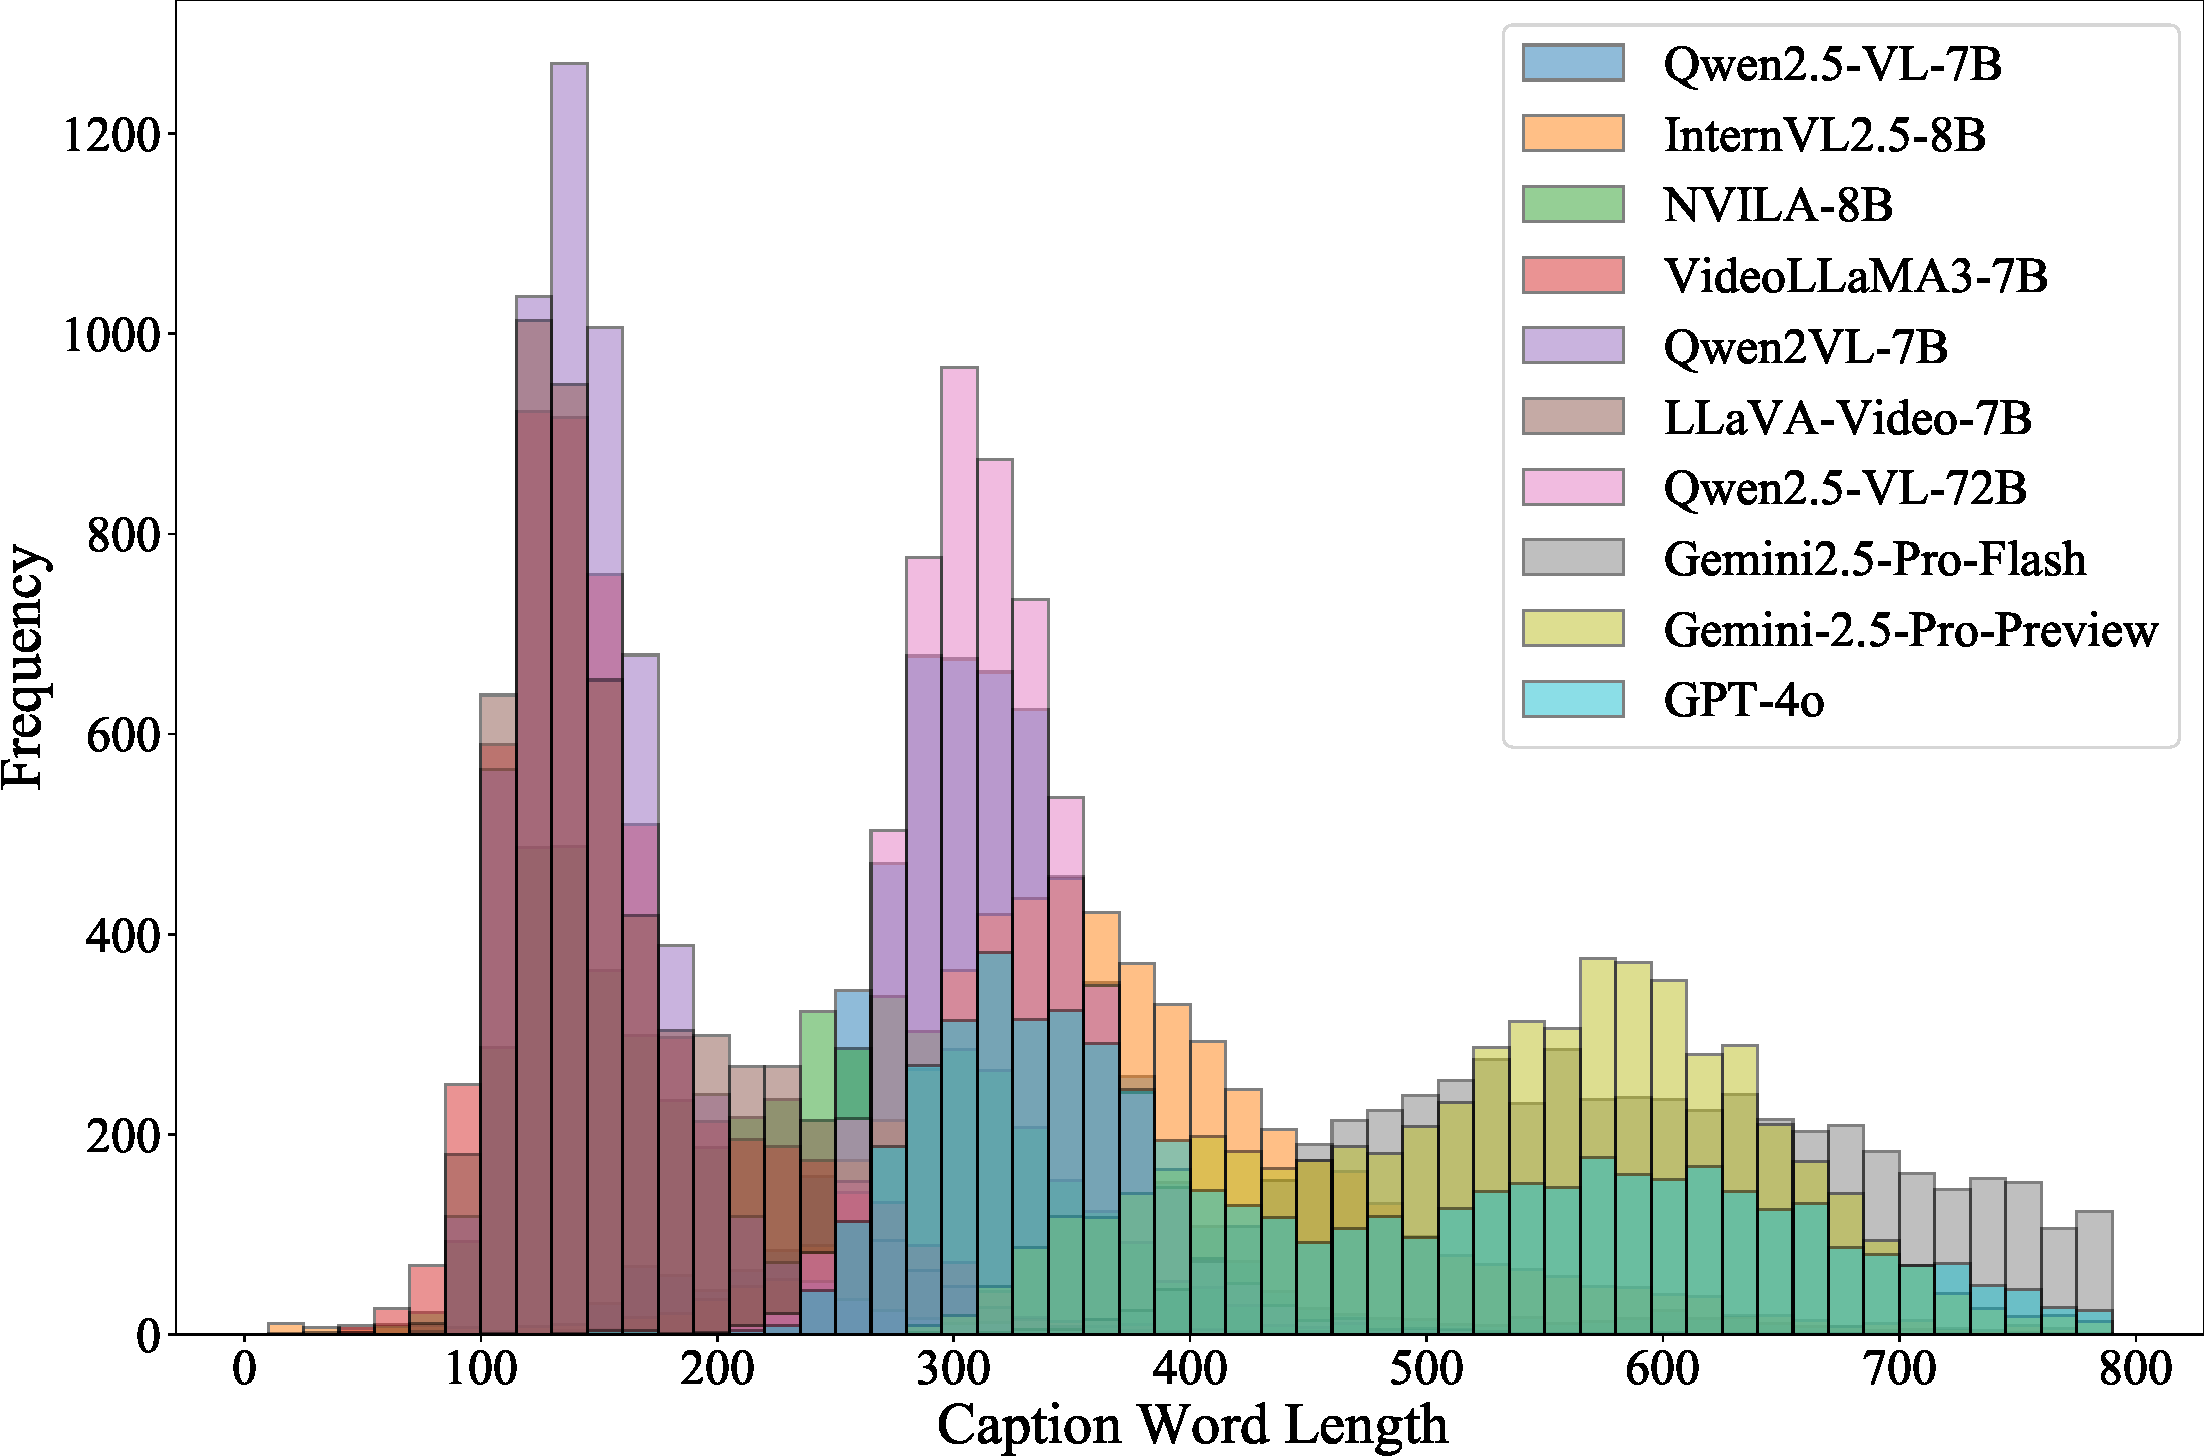
\includegraphics[width=0.9\linewidth]{imgs/word_length_distribution-all-3.pdf}
	\caption{Video caption word length distribution.}
	\label{fig:fig11}
	\end{minipage}%
\end{figure}


Table~\ref{tab:results_2} and Fig.~\ref{fig:fig9} presents the accuracy rate (AR), inconsistency rate (IR), and coverage rate (CR) of various VLM methods across multiple dimensions. Overall, Gemini-2.5-Pro-Preview achieves the best or second-best performance in nearly all categories. Notably, it attains the highest AR and CR in most dimensions, such as ``Background'' and  ``Camera Movement'', reaching 92.72\% and 92.09\%, respectively, which demonstrates its strong multimodal understanding capabilities. Meanwhile, its IR remains low, indicating good consistency in its responses. GPT-4o also shows competitive results in certain aspects (such as ``Entity Shape'' and ``Lighting''), but its overall performance is still slightly behind the Gemini series. In contrast, smaller models like LLaVA-Video-7B and Qwen2VL-7B lag significantly in all metrics, especially in complex scenarios and fine-grained attributes (\eg, ``Blur'' and ``Camera Movement''). In summary, as model scale and multimodal capabilities increase, VLMs exhibit substantial improvements in video understanding tasks, with Gemini-2.5-Pro-Preview currently demonstrating the best overall performance.



Fig.~\ref{fig:fig10} and Fig.~\ref{fig:fig11} compare the performance of various Vision-Language Models (VLMs) in terms of caption length, coverage rate (CR), and inconsistency rate (IR). As shown in Figure 1, advanced models such as Gemini-2.5-Pro-Flash, Gemini-2.5-Pro-Preview, and GPT-4o generate much longer captions and achieve higher coverage rates compared to earlier models like Qwen2VL-7B and VideoLLaMA3-7B. Despite the increase in caption length, the inconsistency rate remains low and stable across all models.

Fig.~\ref{fig:fig11} further illustrates the distribution of caption word lengths. Simpler models tend to produce shorter captions, while the more advanced models generate a wider range of longer captions. Overall, these results indicate that recent VLMs are capable of producing more detailed and comprehensive image descriptions without sacrificing consistency.

\subsection{The Impact of Evaluator Selection on the Results}\label{exp_app1}

\begin{table*}[htbp]
\renewcommand{\arraystretch}{0.6}
\caption{The accuracy (AR), inconsistency rate (IR), and coverage rate (CR) the captions of Gemini-2.5-Pro-Preview, GPT-4o and Qwen2.5-VL-72B, where we compare the results of Gemini-2.5-Pro-Preview, GPT-4o, and Manual comprehensive evaluation. The symbol ``$\uparrow$"  indicates that the larger the value, the better; The symbol ``$\downarrow$" indicates that the smaller the value, the better.}
\label{tab:results_3}
\resizebox{\textwidth}{!}{%
\begin{tabular}{@{}l|ccccccccc@{}}
\toprule
 \multirow{3}{*}{Methods}& \multicolumn{3}{c|}{Gemini-2.5-Pro-Preview}& \multicolumn{3}{c|}{GPT-4o}& \multicolumn{3}{c}{Qwen2.5-VL-72B}\\
 \cline{2-10} 
 & AR$\uparrow$ & IR$\downarrow$ &\multicolumn{1}{c|}{CR$\uparrow$}& AR$\uparrow$ & IR$\downarrow$ & \multicolumn{1}{c|}{CR$\uparrow$} & AR$\uparrow$ & IR$\downarrow$ & CR$\uparrow$  \\
 
 \midrule 
Manual &76.87&9.33&\multicolumn{1}{c|}{87.42} &65.47&13.33&\multicolumn{1}{c|}{74.22} &62.76&11.33&70.27\\
GPT-4o &76.73&10.28&\multicolumn{1}{c|}{85.52} &66.49&10.24&\multicolumn{1}{c|}{74.07} &63.08&10.98&70.86  \\ 
Gemini-2.5-Pro-Preview &73.88&14.62&\multicolumn{1}{c|}{86.52} &63.08&15.90&\multicolumn{1}{c|}{75.01} &61.20&16.02&72.87\\


\bottomrule
\end{tabular}%
}
\end{table*}

We randomly selected 100 samples from the dataset and evaluated the quality of video captions generated by different models (\eg, Gemini-2.5-Pro-Preview, GPT-4o and Qwen2.5-VL-72B) using three methods: manual evaluation, method~b, and method~c. The results are shown in Table~\ref{tab:results_3}. As observed, although there are some differences among the automatic evaluation methods, their results are generally consistent with the manual evaluation, and the performance gaps are not significant. This demonstrates that the proposed automatic evaluation process can effectively support the rapid assessment and optimization of video caption generation models.


\subsection{Limitations}\label{exp_app2}

A primary limitation of our proposed evaluation framework is its dependence on the capabilities of the large language model (LLM) employed as the evaluation expert. The use of different LLMs as evaluators may yield variations in the absolute quantitative scores assigned to model outputs. Nevertheless, as long as the same LLM is consistently used for evaluation and possesses sufficiently advanced capabilities (\eg, GPT-4.1 or Gemini 2.5), it can reliably distinguish the relative quality of video captions generated by different models. In general, the reliability of the evaluation results improves with the strength of the LLM serving as the evaluator. We anticipate that, with the ongoing rapid progress in LLM development, the accuracy and robustness of our automatic evaluation framework will continue to improve, further enhancing its utility for video captioning assessment.
